%\begin{savequote}[75mm]
%Nulla facilisi. In vel sem. Morbi id urna in diam dignissim feugiat. Proin molestie tortor eu velit. Aliquam erat volutpat. Nullam ultrices, diam tempus vulputate egestas, eros pede varius leo.
%\qauthor{Quoteauthor Lastname}
%\end{savequote}

\chapter{The Standard Model and beyond: a theoretical overview}

This chapter presents an overview of the Standard Model of Particle Physics and in particular the physics of the Higgs boson. First, a brief overview of the Standard Model and its history are presented. Then, a description of the Higgs mechanism of electroweak symmetry breaking is given. Next, the physics of single Higgs boson production and decay is described. The Standard Model also allows for production of two Higgs bosons and this is detailed as well. Finally, di-Higgs production in two beyond the Standard Model (BSM) theories - Randall-Sundrum gravitons (RSG) and Two Higgs Doublet Models (2HDM) - is shown. 

\section{The Standard Model of Particle Physics}

The Standard Model (SM) of Particle Physics is a quantum field theory describing the fundamental particles of nature and the forces that govern their interactions. Several comprehensive treatments of the SM already exist in the literature\cite{Griffiths,HalzenAndMartin,Tully,PDG,Schwartz,Dawson} and this section will not rehash those. Rather, this section presents a brief overview of the SM particles and forces in order to define them for subsequent discussions. 

The Standard Model consists of two primary categories of fundamental particles: fermions (spin $1/2$ particles) and bosons (integer spin particles). The SM also describes three forces: electromagnetism, the weak nuclear force, and the strong nuclear force. Gravity is not included in the theory and is largely irrelevant at the scales currently probed by collider experiments. Within the fermions, there are both quarks (which interact via all three forces) and the leptons. The charged leptons interact via electromagnetic and weak interactions, while neutrinos (neutral leptons) interact only via the weak force. Within the bosons, there are the $W^{\pm}$ and $Z$ bosons (the mediators of the weak force), the gluon ($g$, the mediator of the strong force), and the photon ($\gamma$), the mediator of the electromagnetic force. Finally, there is the Higgs boson, a fundamental spin-$0$ particle resulting from the Higgs mechanism of electroweak symmetry breaking.  Figure~\ref{fig:sm_particles} summarizes the fermions and bosons of the SM. 

\begin{figure}[h!]
  %\vspace{20pt}
  \centering
  \captionsetup{justification=centering}

  %\hspace*{-32pt}
  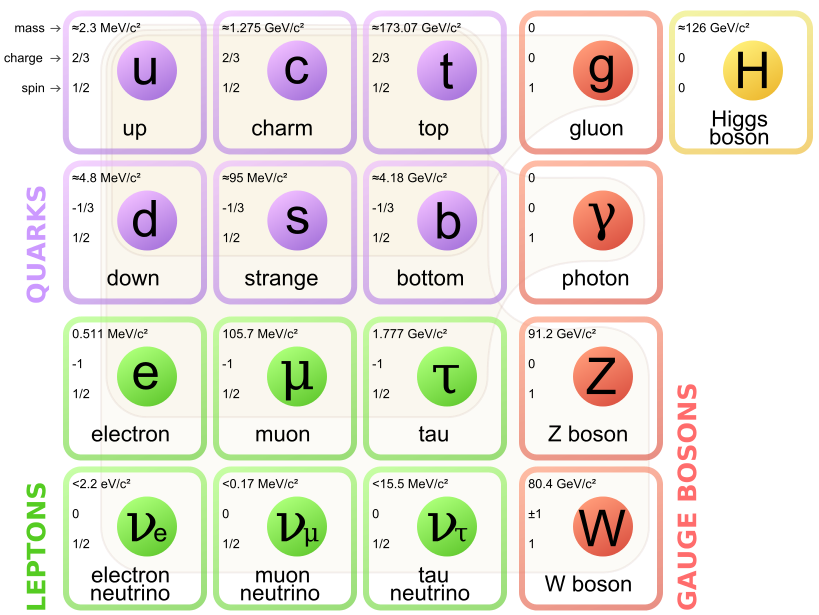
\includegraphics[width=0.6\textwidth]{figures/SM_particles}
  \caption{The particles of the Standard Model and their properties\cite{PDG}.}
  \label{fig:sm_particles}
\end{figure}

The Standard Model coalesced into a unified theoretical framework in the 1960s through the work of Glashow, Weinberg, Salam, and others on the theory of electroweak interactions\cite{Glashow, Weinberg, Salam, Glashow2}. This theory characterized both the electromagnetic and weak interactions as unified under a single gauge symmetry group, namely $SU(2) \times U(1)$. At low enough energy scales (on the order of the $W$ and $Z$ masses, the electroweak symmetry is broken, as evidenced by the fact that the weak bosons have mass while the photon does not. The discovery of the Higgs boson in 2012 confirmed the Higgs mechanism as the most likely candidate for this electroweak symmetry breaking\cite{Discovery, CMSDiscovery}. The electroweak theory is then combined with the theory of quantum chromodynamics (which models the strong sector as a non-abelian $SU(3)$ gauge group) to form the complete SM\cite{QCDBook}. 

\section{Electroweak Symmetry Breaking and the Higgs}

In the Standard Model Lagrangian, it is difficult to include mass terms for the $W$ and $Z$ bosons without breaking the fundamental gauge symmetry of the Lagrangian. A traditional mass term does not preserve the $SU(2) \times U(1)$ symmetry. Additionally, scattering of massive $W$ and $Z$ bosons violate unitarity and these diagrams diverge at high energy scales. In the 1960s, Higgs, Brout, Englert, Guralnik, Kibble, and Hagen developed a mechanism for spontaneous symmetry breaking via the additioanl of a complex scalar doublet to the SM. Three of the four real degrees of freedom of this complex field would go to the longitudinal modes of the $W^{\pm}$ and $Z$, thus allowing them to have mass\cite{Higgs1,Higgs2,Englert,Guralnik}. The remaining degree of freedom would manifest as an additional scalar, known now as the Higgs boson (Higgs was the first to predict the existence of the new particle). 

The mechanism works by introducing a Lagrangian for the newly introduced field that still respects the symmetry of the Standard Model inherently, but with a minimum at a non-zero vaccuum expectation value for the field. In this minimum of the potential, the electroweak symmetry is broken. Specifically, consider a complex scalar doublet $\phiH$ with four degrees of freedom, as shown in equation~\ref{eqn:phi_def}.

\begin{equation}
\label{eqn:phi_def}
\phiH = \left( \begin{array}{c} \phi^+ \\ \phi^0 \end{array} \right) = \frac{1}{\sqrt{2}}\left( \begin{array}{c} \phi_{1}^{+} + i\phi_{2}^+ \\ \phi_1^0 + i\phi_2^0 \end{array} \right)
%\phiH = \left( \begin{array}{c} \phi^+ \\ \phi^0  \end{array}\right) = \left( \begin{array}{c} \phi_1^+ + i\phi_2^+ \\ \phi_1^0 + i \phi_2^0 \end{array}\right) 
\end{equation}

The minimal potential of a self-interacting Higgs that still respects the SM symmetry is given in equation~\ref{eqn:potential}.

\begin{equation}
\label{eqn:potential}
V(\phiH) = \mu^2 \phiH^{\dagger}\phiH + \lambda(\phiH^\dagger\phiH)^2
\end{equation}

If the $\mu^2$ term of this potential is positive, then the potential has a minimum at $\phiH = 0$ and the SM symmetry is preserved. However, if instead $\mu^2 < 0$, then the minimum is at a finite value of $\phiH$, namely

\begin{equation}
\phiH_{\rm min} = \frac{1}{\sqrt{2}} \left(\begin{array}{c} 0 \\ v\end{array} \right)
\end{equation}

where $v = \sqrt{\mu^2/\lambda}$. Because this is the location of the minimum, it corresponds to the vacuum expectation value for the field ($\langle\phiH\rangle = \phiH_{\rm min}$). The excitations of the Higgs can then be parameterized as 

\begin{equation}
\phiH = \frac{1}{\sqrt{2}} \left(\begin{array}{c} 0 \\ v + H \end{array}\right)
\end{equation}

The full scalar Lagrangian, including the kinetic term, is then given as 

\begin{equation}
\mathcal{L}_s = (D^\mu \phiH)^\dagger(D_\mu\phiH) - V(\phiH)
\end{equation}

where the covariant derivative is defined as 

\begin{equation}
D_\mu = \partial_\mu + \frac{ig}{2}\tau^aW_\mu^a + ig'YB_\mu
\end{equation}

and $W^1, W^2, W^3$ and $B$ are the $SU(2)$ and $U(1)$ gauge fields of the electroweak theory, respectively. $g$ and $g'$ are the corresponding coupling constants. With the scalar Lagrangian in place, the physical gauge fields can then be written as 

\begin{equation}
\label{eqn:Weq}
W_\mu^\pm = \frac{1}{\sqrt{2}}(W_\mu^1 \mp iW_\mu^2) 
\end{equation}

\begin{equation}
\label{eqn:Zeq}
Z_\mu = \frac{-g'B_\mu + gW_\mu^3}{\sqrt{g^2 + g'^2}} 
\end{equation}

\begin{equation}
\label{eqn:photoneq}
A_\mu = \frac{gB_\mu + g'W_\mu^3}{\sqrt{g^2 + g'^2}}
\end{equation}

Equation~\ref{eqn:Weq} corresponds to the charged $W^+$ and $W^-$ bosons, equation~\ref{eqn:Zeq} corresponds to the neutral $Z$ boson, and equation~\ref{eqn:photoneq} corresponds to the neutral photon. The masses of the particles also arise from the Lagrangian. The photon has zero mass, while the masses of the $W$ and $Z$ bosons are given in equation~\ref{eqn:bosonmasses}.

\begin{equation}
\label{eqn:bosonmasses}
\begin{array}{c}
M_W^2 = \frac{1}{4}g^2v^2 \\ 
M_Z^2 = \frac{1}{4}(g^2 + g'^2)v^2
\end{array}
\end{equation}

The fermion masses also arise through a coupling with the Higgs via the Yukawa interaction (for a detailed description, see\cite{Dawson}). In this case the coupling between the Higgs and the fermions goes as 

\begin{equation}
\label{eqn:higgs-fermions}
g_{Hf\bar{f}} = \frac{m_f}{v}
\end{equation} 

The full Lagrangian of Higgs interactions can be written as 

\begin{equation}
\mathcal{L}_{\rm Higgs} = -g_{Hf\bar{f}}\bar{f}fH + \frac{g_{HHH}}{6}H^3 + \frac{g_{HHHH}}{24}H^4 + \delta_V V_\mu V^\mu\left(g_{HVV} H + \frac{g_{HHVV}}{2}H^2\right)
\end{equation}

with 

\begin{equation}
\begin{array}{cc}
g_{HVV} = \frac{2m_V^2}{v} & g_{HHVV} = \frac{2m_V^2}{v^2} \\ 
g_{HHH} = \frac{3m_H^2}{v} & g_{HHHH} = \frac{3m_H^2}{v^2}
\end{array}
\end{equation}

Here, $V$ refers to the $W^{\pm}$ and $Z$, and $\delta_{W} = 1$ while $\delta_Z = 1/2$. Phenomenologically, there are a few features of this Lagrangian that are useful to note. First, note that the Higgs mass is a free parameter of the theory that must be determined experimentally. Second, note that the coupling of the Higgs to the vector bosons and fermions scales with the masses of these particles, a fact that is important when considering both the production and decays of the particle. Also note that the branching ratio of the Higgs to $W$ bosons will be twice that of the branching ratio to $Z$ if the Higgs mass is large enough to produce the particles on shell because of the extra symmetry factor associated with the $W$ coupling. Finally, note the presence of the cubic and quartic Higgs self interaction terms, which can lead to final states with multiple Higgs bosons produced. 

\section{Higgs Boson Production and Decay}

\section{Higgs Pair Production in the Standard Model}

\section{Higgs Pair Production in Theories Beyond the Standard Model}


% For an example of a full page figure, see Fig.~\ref{fig:myFullPageFigure}.

%\texttt{This is a line of code.}

%\begin{figure}
%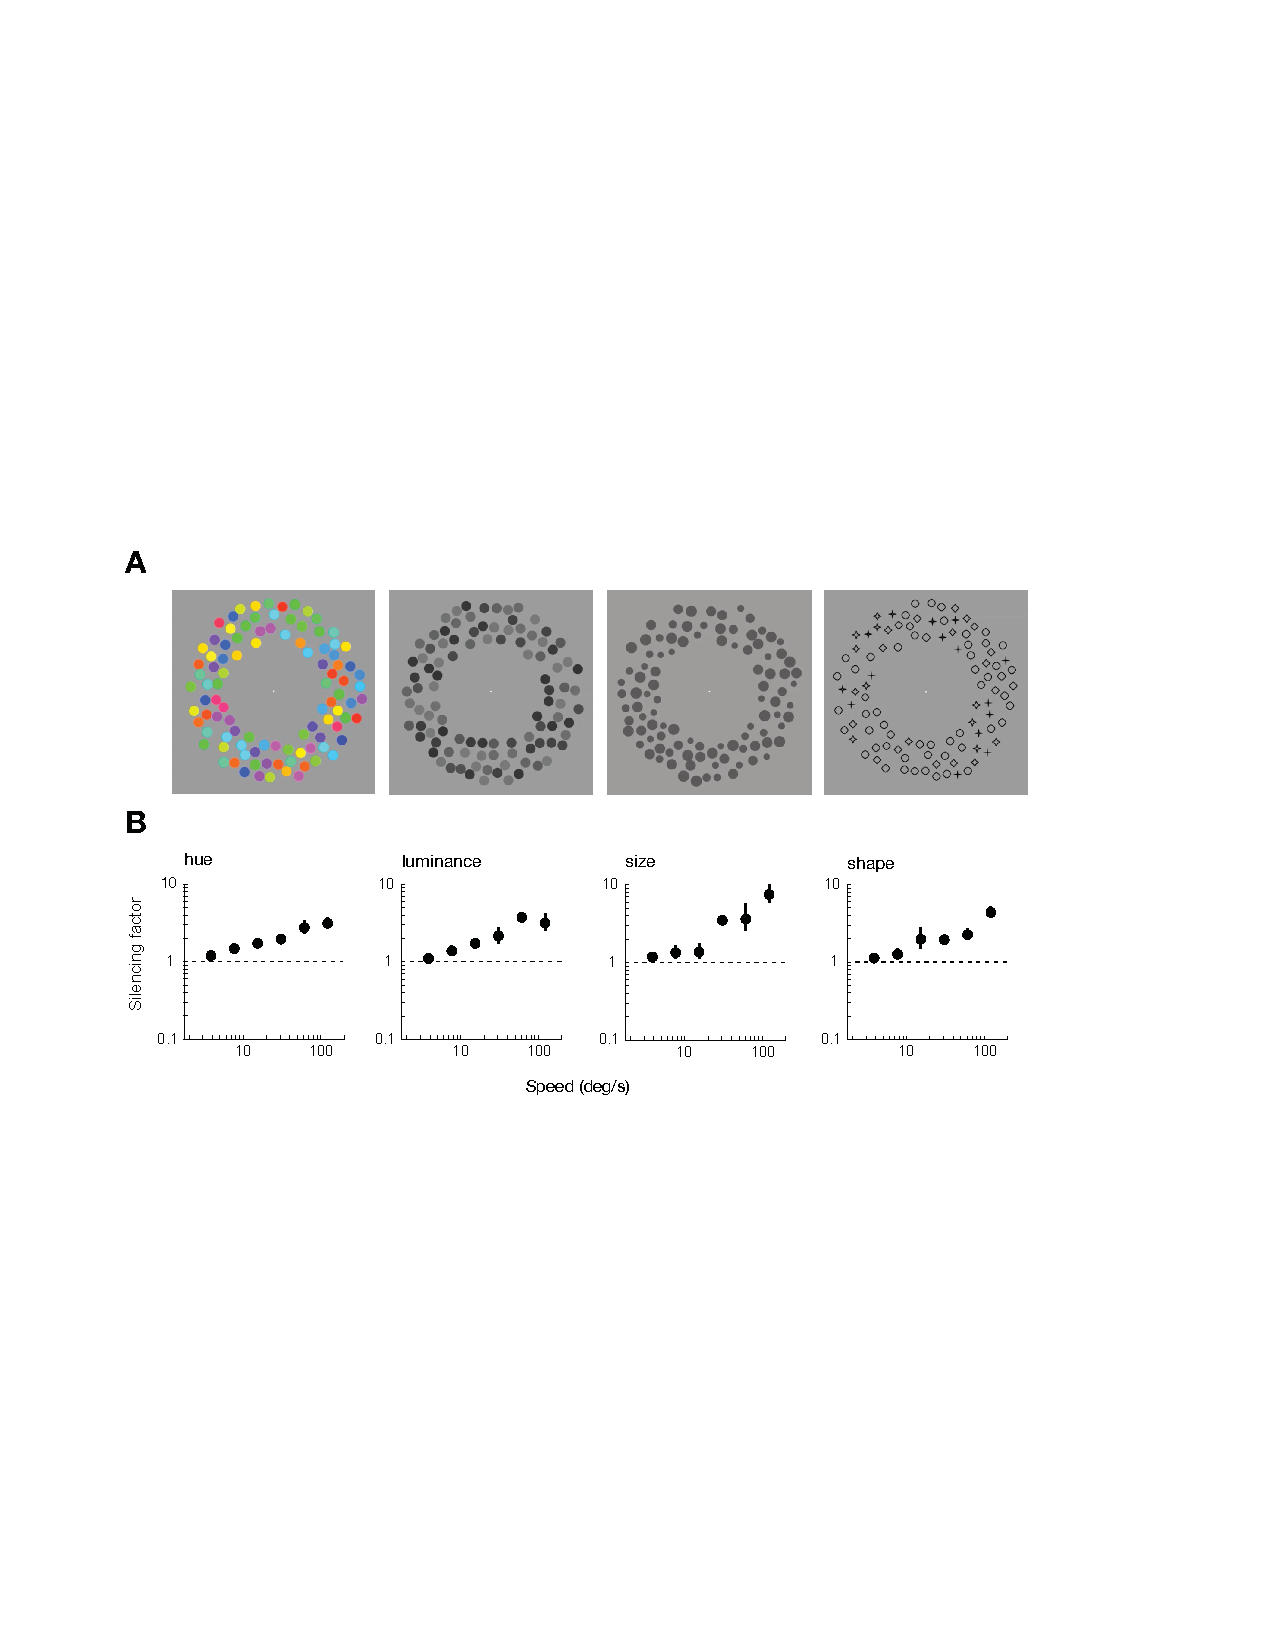
\includegraphics[width=\textwidth]{figures/fig1}
%\caption[Short figure name.]{This is a figure that floats inline and here is its caption.
%\label{fig:myInlineFigure}}
%\end{figure}

%% Requires fltpage2 package
%%
% \begin{FPfigure}
% 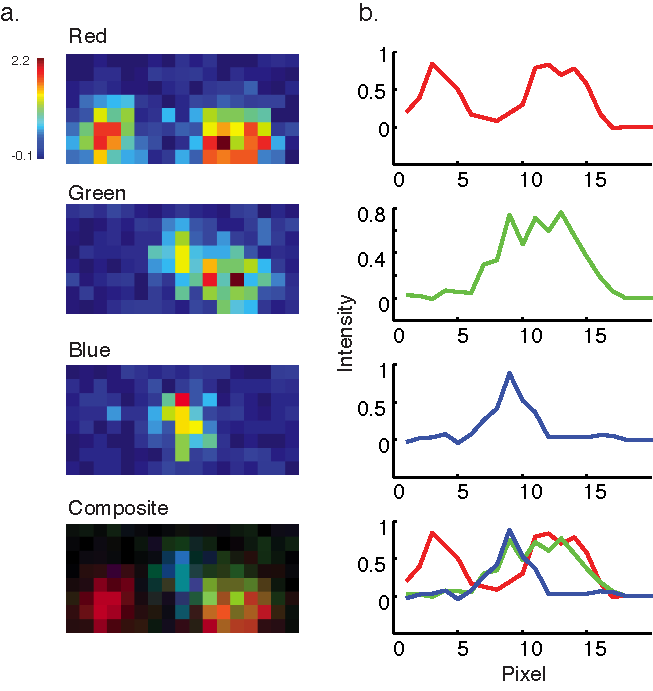
\includegraphics[width=\textwidth]{figures/fullpage}
% \caption[Short figure name.]{This is a full page figure using the FPfigure command. It takes up the whole page and the caption appears on the preceding page. Its useful for large figures. Harvard's rules about full page figures are tricky, but you don't have to worry about it because we took care of it for you. For example, the full figure is supposed to have a title in the same style as the caption but without the actual caption. The caption is supposed to appear alone on the preceding page with no other text. You do't have to worry about any of that. We have modified the fltpage package to make it work. This is a lengthy caption and it clearly would not fit on the same page as the figure. Note that you should only use the FPfigure command in instances where the figure really is too large. If the figure is small enough to fit by the caption than it does not produce the desired effect. Good luck with your thesis. I have to keep writing this to make the caption really long. LaTex is a lot of fun. You will enjoy working with it. Good luck on your post doctoral life! I am looking forward to mine. \label{fig:myFullPageFigure}}
% \end{FPfigure}
% \afterpage{\clearpage}


